\section{Prototyping}

Nachdem ein Gesamtkonzept geplant wurde, wird nun möglichst viel Prototyping durchgeführt. Das Ziel ist es, zu testen, ob das ermittelte Konzept funktionieren könnte oder ob es überarbeitet werden muss. So kann mit den Risiken, die im vorhergehenden Kapitel ermittelt wurden, besser umgegangen werden.

\subsection{...}

\subsection{Kürzester Weg finden}

Da es nur 8 Knoten im Graph gibt, wurde von Anfang an vermutet, dass die Geschwindigkeit des Algorithmus vernachlässigt werden kann.

Um zu überprüfen, dass diese These stimmt, wurde ein traditioneller Dijkstra Algorithmus in Python implementiert. Dabei wurde von einem Knoten der kürzeste Weg zu allen anderen Knoten im vorgegebenen Graphen mit 8 Knoten berechnet. Die Zeit dafür wurde gestoppt und ausgegeben:

TODO: Skript anhaengen oder verlinken?

\begin{figure}[H]
\centering
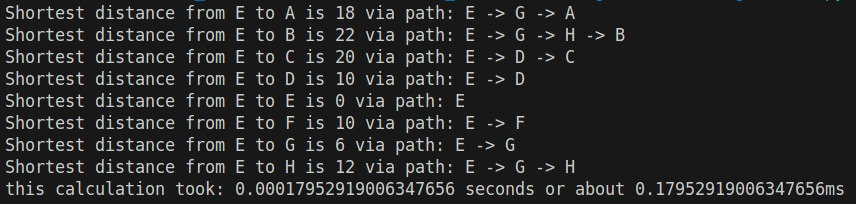
\includegraphics[width=\textwidth -30mm]{assets/informatik-prototyp/dijkstra-time.jpeg}
\caption{Dijkstra Zeitmessung}
\label{fig:dijkstra-time}
\end{figure}

Um den kürzesten Pfad acht mal zu berechnen wurden ungefähr 0.18 ms benötigt. Dies ist schnell genug. Aufgrund dieses Test wurde entschieden einen einfachen selbst implementieren Dijkstra zu verwenden, da es wichtig ist, dass der Algorithmus möglichst lightweight ist, da nur beschränkte Rechenkraft und Speichergrösse zu Verfügung stehen.


\subsection{Bilderkennung}

\subsubsection{Spiegelung}

spiegelt stark, vor allem Problem, um Knoten zu erkennen; Bilder entspiegeln: Lichtverhaeltnisse, Polfilter oder Nachbearbeitung.\cite{avoid-reflection}

\subsubsection{YOLOv11}

Auf Roboflow\footnoe{https://roboflow.com/} Bilder labeled:

TODO BILD

Mihilfe eines Jupyter skripts 

\subsection{Simulator}

TODO: eigenes File?

Das Erarbeiten des Konzeptes des Simulators, der Implementierung und des Gebrauchs wird in diesem Kapitel festgehalten.

Nach der Nutzwertanalyse war das grundlegende Konzept klar und es konnte mit der Implementierung begonnen werden.

- GitHub, Issues sammeln, Festlegen Git ettiquete (aka MRs)

- Struktur mit Klassen (ERD?): Robot, Reader, Calculator, GUI

- Roboter liest Graph, ueberprueft Nodes und Barrieren

- Calculator holt kürzester Weg, Roboter geht zu nächsten Node

- Poetry

- Die einzelnen Kanten werden identifiziert mit Sortierung

- GUI Roboter bewegt sich
